\chapter{提案手法2}\label{method2}
\ref{mip}章で,現実的な時間で実行可能解を出力することのできる問題例の規模を確認した.

より大規模な問題例を現実的な時間で解くために,ヒューリスティックを用いた数理モデルを提案する.

\section{ホールドの統合}
本研究では,ホールドの数が43の運搬船を考えている.
実オペレーションでは,それぞれのホールドを個別で考えるのではなく,複数のホールドをある程度まとめて考えて作業を行っている.
そのため,各階においてスロープのついているホールドを境目として,2つのホールドのまとまりとして考える.

複数のホールドを1つのまとまりとして考えると,43のホールドを,17のまとまりに統合することができる.このまとまりをセグメントと呼び,具体的な統合については
図\ref{fig1}に示す.\\

\begin{figure}[H]
 \centering
 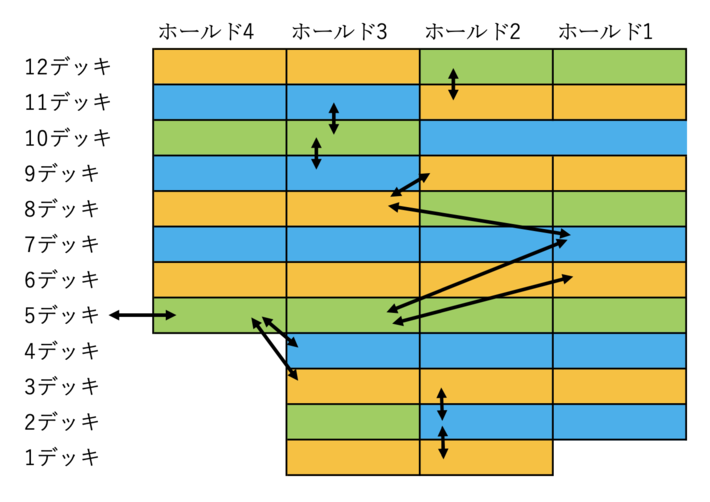
\includegraphics[slace=0.2]{segment.png}
 \caption{統合後のホールドを色付けしたもの}
 \label{fig1}
\end{figure}



\section{解の表現方法}
鵜川らによる研究の数理モデル\cite{ukawa}では,ホールドに注文を何台割り当てる,という連続的な解の表現方法を用いていた.
ヒューリスティックモデルでは,このような連続的な解表現方法を用いず,注文のセグメントへの割当のみを最適化し,詳細な車両の積載は決め打ちのルールを基に行っていく.
積載のルールは,ホールドの積載可能量,許容充填率などを満たすように設計を行っていく.

このように積載貨物を決めていくことで,注文を複数のホールドに渡って分割する場合であっても,隣接したホールドに車両を積むことができるため,プランナーの考える割当に近い解を出力することができる.

\section{局所探索法}
局所探索法とは, ある解に少しの変更を加え得た近傍解が元の解よりも良い解である場合に, 変更後の解に移動するという操作を良い解が見つからなくなるまで繰り返す方法である.
変形を加える操作を近傍操作と呼び, 近傍内に改善解を持たない解を局所最適解と呼ぶ.

本研究では,初期解を生成した後に局所探索法を用いて解の改善を行う手法を提案する.
また,評価関数として鵜川らによって提案された目的関数\cite{ukawa}を用いる.
また,貨物の重量バランスに関する制約などに違反している場合には,制約違反度合いをペナルティ関数として表し, 目的関数に加えて探索を行う.

\section{初期解の生成}
\label{initial}
局所探索における初期解の生成方法として,2種類のアプローチを提案する.
\subsection{整数計画問題の緩和解の利用}
\label{relaxation}
定式化を行った整数計画問題の整数制約を緩和した線形緩和問題の解を初期解として利用することを考える.
この手法は,有効な解が得られたことが確認できている整数計画問題の解と線形緩和問題の性質が似ている場合に有効であると考えられる.
予備実験としてハミング距離を用いてそれぞれの解の性質を比較する.

\subsubsection{ハミング距離}
ハミング距離とは,2つのベクトルの各要素の比較を行い,異なる要素の数がどの程度あるかを示すものである.

長さ$n$の0-1ベクトル$x,y$に対して,ハミング距離$d_H$は一般的に以下のように定義される.
\begin{align*}
 d_H(x,y) =\sum_{i=1}^n |x_j-y_i|
\end{align*}

\subsubsection{ハミング距離の計算方法}
本研究では,各注文におけるホールドへの割当台数を目的変数としている.
各注文における車両台数は異なるため,ハミング距離を計算するためには正規化をする必要がある.

注文における車両台数のなかで,特定のホールドに割り当てる注文台数の割合を変数とすると,0から1の値を必ずとることがわかる.
各注文において,注文が全て割り当てられていれば和は1になる.

整数計画問題の解と線形緩和問題の解をそれぞれ正規化したベクトルを$x,y$とする.
注文数を$n$,ホールドの数を$m$としたとき,ハミング距離を以下のように計算する.
\begin{align*}
 d_H(x,y) =\sum_{i=1}^n \sum_{j=1}^m|x_{ij}-y_{ij}|
\end{align*}
注文の全てが割り当てられている場合にハミング距離の和は$2n$になるため,$2n$で割ると2つの解の性質がどの程度異なるかを測ることができる.


\subsubsection{線形緩和問題の解の性質}
整数計画問題の解と線形緩和問題の性質の比較を行う.
解の精度が十分に良いことがわかっている解で比較を行う必要があるため,整数計画問題において厳密解が出た問題例で比較を行い,結果を表\ref{hamming}に示す.

どのインスタンスにおいても,整数計画問題の解の性質に近い線形緩和問題の解が存在することが確認できた.

\begin{table}[h]
  \centering
  \caption{線形緩和問題の解との比較}
  \label{hamming}
\begin{tabular}{cccr}
\hline
注文数 & 積み地 & 揚げ地 & \multicolumn{1}{c}{解の差異(\%)} \\ \hline
38 & 2   & 3   & 0.19                        \\
38 & 2   & 3   & 3.57                         \\
57 & 2   & 5   & 1.07                         \\
66 & 4   & 3   & 0.71                        \\ \hline
\end{tabular}
\end{table}

\subsubsection{線形緩和解の丸め方}
線形緩和問題では,注文のホールドへの割当として小数点が出てくる場合がある.
各注文を,緩和解の変数値の最も大きいホールドに割り当てると一部のホールドに大量に割り当てられる解が出る可能性があるため,割り当てられた値を確率として,その確率を基にランダムに割り当てる手法で初期解を生成する.
ただし,割り当てるホールドの容量制約が満たされない場合には,そのホールドには割り当てない.


\subsection{港が同じ注文をまとめて席割を作成}
\label{model2}
鵜川らは,注文の積み地と揚げ地が同じ注文を1つのグループとして考え,グループ化された注文をホールドに割り当てることで計算時間を短縮する手法を提案した\cite{ukawa}.
解の精度としては,ある程度有効ではあるものの,実際に利用するためには修正が必要であった.

本研究では,この手法で得られた解を局所探索における初期解として利用するアプローチを提案する.


\section{近傍操作}
近傍操作には挿入近傍操作と交換近傍操作を用いる.

挿入近傍操作は,セグメントに割り当てられている注文の1つを,ランダムに異なるセグメントに挿入する操作である.
交換近傍操作は,異なるセグメントに割り当てられている注文を2つランダムに選び,それらを入れ替える操作である.

本研究では,はじめに挿入近傍操作を改善がなくなるまで繰り返し,その後交換近傍操作を改善がなくなるまで行う.
挿入近傍操作で1回でも改善があった場合は,再び挿入近傍操作からやり直す.


\subsection{計算時間の短縮}
\label{近傍操作の計算時間短縮}
本研究では,局所探索における近傍操作の1つとして挿入近傍操作を用いるが,操作に工夫を加えることで解の精度を変化させることなく計算時間を短縮させることができると考えられる.

挿入近傍操作では,1つの注文を異なるセグメントに挿入する.その際に,挿入可能な位置すべてを探索し評価関数の値が最も良くなる位置に挿入する.

しかし,あるセグメントに格納される注文の順番が変化しても評価関数の値が全く変化しない場合がある.そのような場合にはすべての挿入可能位置を探索する必要がないため,計算時間を短縮することができる.

以下に計算時間を短縮する提案手法の概要を示す.

\begin{algorithm}
 \caption{計算時間を短縮する手法}
 \label{algo1}
 \begin{algorithmic}[1]%1を0にすると行番号なし.
  \STATE あるセグメントから,注文を1つ選択する
  \STATE 挿入先のセグメントの,一番最後の位置に挿入する
  \STATE 複数のセグメントに分割された注文を$J_{\rm split}$とする.
  \FOR {$j \in J_{\rm split}$}
  \STATE $j$の前後に注文を挿入する
  \IF {評価関数の値が暫定解よりも良い}
  \STATE 暫定解を更新
  \ENDIF
  \ENDFOR
  \IF {暫定解が探索における最良解よりも良い}
  \STATE 最良解を更新
  \ENDIF
 \end{algorithmic}
\end{algorithm}
